%%%%%%%%%%%%%%%%%%%%%%%%%%%%%%%%%%%%%%%%%%%%%%%%
\input{preamble.ltx}

% correct bad hyphenation here; separate each word by a space
\hyphenation{op-tical net-works semi-conduc-tor}

%%%%%%%%%%%%%%%%%%%%%%%%%%%%%%%%%%%%%%%%%%%%%%%%
\begin{document}

\title{Bluetooth Enabled Panic Button for Potential Rape Victims}

\author{
	{\small
		%\renewcommand{\arraystretch}{1.3}
		\begin{tabular}{l l l}
			& \multicolumn{2}{c}{\tiny \textcolor[rgb]{0.9,0.9,0.9}{Participated in \& did the coursework [Y/N]?}} 
			\\ 
			GUEVARRA,~Alnair~M.~(11524855) & Y & 
\includegraphics[height=5ex] {A_signature} 
			\\ 
			HERNANDEZ,~Roy~Stephen~A.~(11530731)     & Y & 
\includegraphics[height=5ex]{R_signature}
			\\ 
			LAGMAN,~Maria~Josefa~M.~(11531029)  & Y & 
\includegraphics[height=5ex]{mama_signature} 
			\\
			MOLINA,~Adam~M.(11539607)  & Y & %\includegraphics[height=5ex]{Capture1}
			\\  		
		\end{tabular}
	}
% for author names; note positions of commas and nonbreaking spaces ( ~ ) LaTeX will not break a structure at a ~ so this keeps an author's name from being broken across two lines.
\thanks{\CrmD\protect\\} %<--Do not delete this \thanks{\CrmD\protect\\} 
 \thanks{Coursework Starting Date: \hspace{1ex} July 13, 2018}
\thanks{Submission Date: \hspace{1ex} August 18, 2018}} 

\markboth{\makebox[\columnwidth]{DIGCOMM Project \hfill}%
\hspace{\columnsep}\makebox[\columnwidth]{\hfill}}%
{} % header

\IEEEpubid{\makebox[\columnwidth]{DIGCOMM - EK \hfill DLSU}%
\hspace{\columnsep}\makebox[\columnwidth]{ \hfill {\tiny\textcolor[rgb]{0.4,0.4,0.4}{\prsDy}}}} % footer

\maketitle % for making the title area


\section{Conspectus}
\label{sec:cnspcts}

\IEEEpubidadjcol % needed in second column of first page if using \IEEEpubid

\subsection{What are the objectives of the coursework?}
\begin{enumerate}
	\item To assess any Digital Communications Technology (DCT) to be used in marginalized sector.
	\item To modify the DCT appropriate to the selected marginalized sector.
	\item To appraise the economic, societal, and environmental implications of the modified DCT.
\end{enumerate}	

\subsection{How does the coursework fit with the course and previously done coursework?}
By:
\begin{enumerate}
	\item Involving the modification of a communication platform between potential rape victims and emergency contacts
	
	\item Using digital communications theory to enhance performance of data transmission for the protection of app users.
	
\end{enumerate}	

\subsection{How were the objectives achieved?}
By:
\begin{enumerate}
	\item Targeting the marginalized sector of the DCT which are potential rape victims.
	\item Modifying the multiple access method used by bluetooth from FH-CDMA to TDMA
	
\end{enumerate}

\subsection{What are the key results and generalizations?}
The key results are:
\begin{enumerate}
	\item To help the master (rape victim) in a Piconet maintain more than one connection simultaneously.
	\item make use of multiple point in reaching out contacts once the panic button is pressed.
	\item modification of multiple access scheme used by bluetooth standard.

\end{enumerate}

\section{Concepts and Principles}
\label{sec:concps}

\subsection{What are the necessary and relevant concepts and principles for understanding the coursework and for supporting the correct results?}
\begin{enumerate}
	\item Mastery of how Bluetooth works and its specifications
	\item Knowledge about different techniques used in Multiplexing methods
	\item Clear understanding of Frequency Hopping Spread Spectrum (FHSS)
	\item Basic concepts about bluetooth connections
	
\end{enumerate}

\subsection{How does any new component, not covered in  previous coursework, function?}
By:
\begin{enumerate}
	\item Overlaying Time Division Multiplexing (TDM) on bluetooth connections. 
	
	\item Incorporating frequency hopping with TDM for simultaneous data transmission
	
	\item Synchronizing a master device with the other two devices through the use of frequency hopping.
	
\end{enumerate}


\subsection{What figures, equations, and/or tables could support your answers in Sec. 2.1 and Sec.2.2?}
\begin{enumerate}
	\item The figure below shows an example of a wireless connection between a single or multiple devices using bluetooth
	\begin{figure}[hp]
		\centering
		\captionsetup{justification=centering,margin=2cm}
		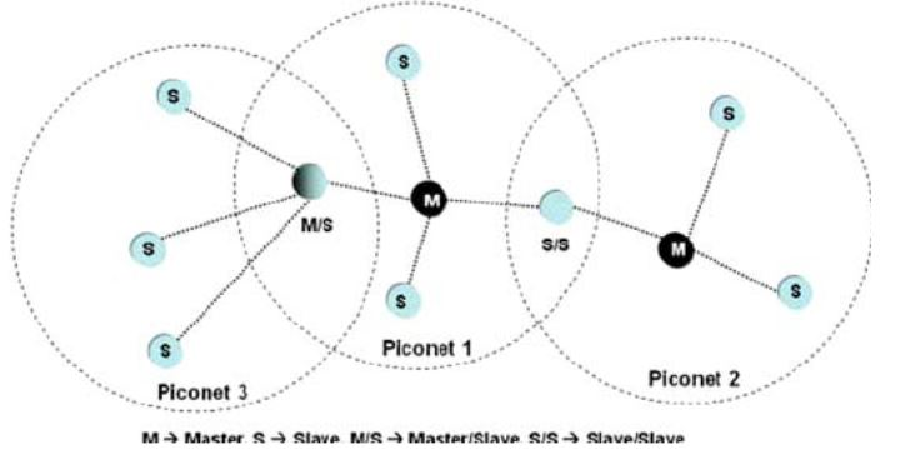
\includegraphics[height=25ex]{piconet}
		\caption{Piconet}
	\end{figure}
	\item The figure below shows a block diagram implementation for frequency hopping code.
	\begin{figure}[ht]
		\centering
		\captionsetup{justification=centering,margin=2cm}
		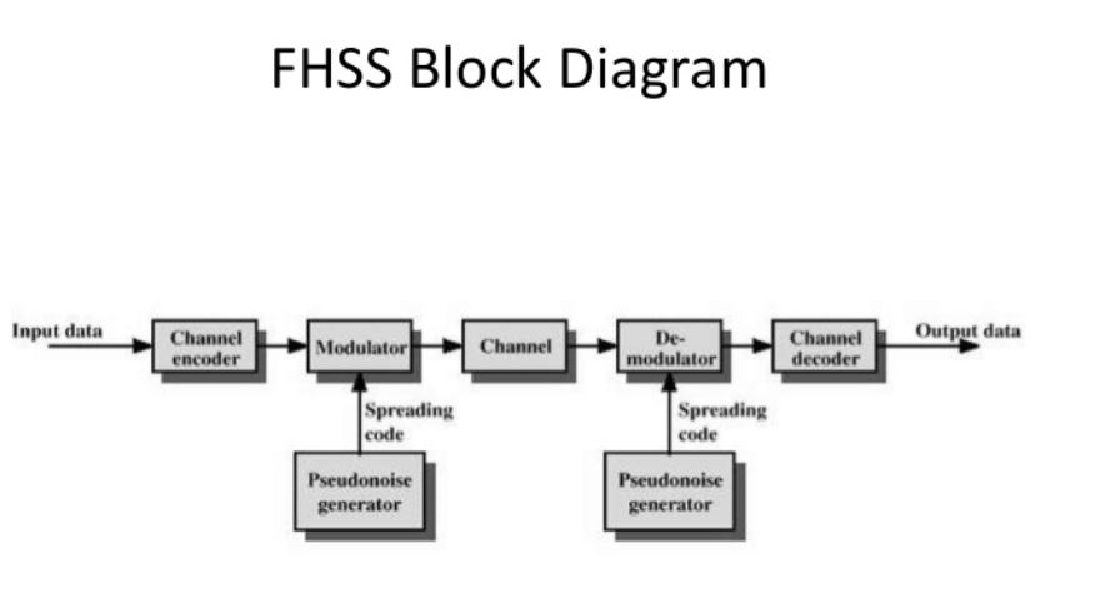
\includegraphics[height=30ex]{fhss}
		\caption{Block Diagram of FHSS}
	\end{figure}
\end{enumerate}

\subsection{Did you cite more than two publications in your answers in Sec. 2.1. and 2.2}
Yes
	
\subsection{Did you cite any online source in your answers in Sec.2.1 and Sec.2.2?}
Yes.


\section{Methodology}

\subsection{How does your implementation in Sec.~\ref{sec:implem} achieve the objectives?}
By:
\begin{enumerate}
	\item Simulating the performance difference between CDMA and TDMA.
	\item Showing application of TDM and full full duplex transmission to panic button device.
\end{enumerate}

\subsection{Why does your implementation in Sec.~\ref{sec:implem} achieve the objectives?}
Because:
\begin{enumerate}
	\item The application of TDMA simplifies the point to multiple-point connections
	
	\item Multiple-point connections can help the rape victim reach out to a lot of contacts simultaneously
	
\end{enumerate}

\subsection{How does your evaluation in Sec.~\ref{sec:eval} achieve the objectives?}
By:
\begin{enumerate}
	\item Achieving these results, it can be proven that the use of overlay TDM into FSHH would improve its duplexing technique.
	\item it would make the panic button device more efficient and faster for reaching help since multiple contacts are accessed simultaneously.
\end{enumerate}

\subsection{Why does your evaluation in Sec.~\ref{sec:eval}  achieve the objectives?}
Because:
\begin{enumerate}
	\item 
	It is proven that a possibility of simultaneous access point is possible with bluetooth through simulation
	
	\item It could serve as new innovation to further studies about multiple access with bluetooth.
\end{enumerate}



\subsection{Implementation}
\label{sec:implem}

\subsubsection{What were the materials used?}
\begin{enumerate}
	\item Bluetooth Module
	\item Arduino
	\item Push Button
\end{enumerate}


\subsubsection{What is the summary of the processes used to make the coursework?}

\begin{figure}[hp]
	\centering
	\captionsetup{justification=centering,margin=2cm}
	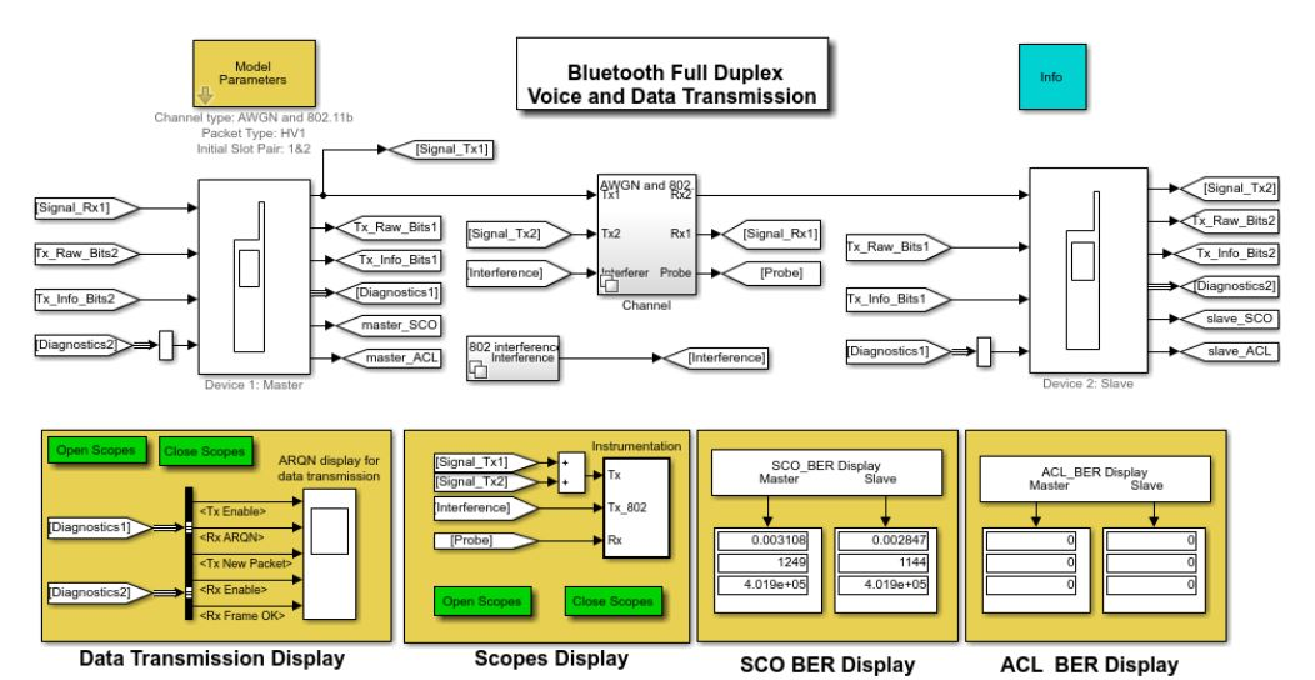
\includegraphics[height=30ex]{bluetoothsimulink}
	\caption{An example of bluetooth module in SIMULINK to be used for DCT}
\end{figure}

\begin{enumerate}
	\item Overlaying of bluetooth protocol to hardware device.
	\item Master device shares different hopping code for each slave devices.
	\item Each slave devices are independent of each other.
\end{enumerate}

\subsection{Evaluation}
\label{sec:eval}

\subsubsection{What were your procedures for evaluating the correct outcome of your coursework?}
\begin{enumerate}
	\item researched for different multiplexing techniques.
	\item studied the difference between FHSS and TDMA and how TDMA was incorporated to bluetooth.
	\item creating a full duplex piconet between a master and slave device for comparison.
\end{enumerate}

\subsubsection{What quantities were gathered and how have you obtained them for testing the veracity of your results?}
\begin{enumerate}
	\item Hopping Spectrogram
	\item Timing Diagram
	\item BER Calculation Rate
\end{enumerate}


\section{Results and Discussions}

\subsection{How do the results achieve the objectives?}
By:
\begin{enumerate}
	\item Showing that TDMA was more efficient compared to CDMA. With this, the modified DCT would highly benefit the marginalized sector.
	\item Showing that TDM and FDM overlays protocol are beneficial to helping the device to be able to connect to more than one data connection to other devices simultaneously;
	\item From the aforementioned statement, it showed that using bluetooth modules with modified DCT, is better than using other modules such as GSM/GPRS because the marginalized sectors are able to get more with less expenses.
	
\end{enumerate}

\subsection{Why do the results achieve the objectives?}
Because:
\begin{enumerate}
	\item Up to two lines per item.
	\item Up to two lines per item.
\end{enumerate}

\subsection{Are all you results correct  in accordance to what you described in Sec.~\ref{sec:eval} evaluation process? Why?} 
Yes/no, because:
\begin{enumerate}
	\item Up to two lines per item.
	\item Up to two lines per item.
\end{enumerate}

\subsection{What is result $X$ (briefly describe it here), what does it mean if it is correct, and how does it contribute in reaching the objectives?}
\label{sec:resn}

\begin{enumerate}		
	\item Refer to the appropriate caption number  of your result, i.e. Fig.~$X$ for figure $X$, Table~$X$ for table $X$, etc.	
	\item Interpret result $X$ and the reasons why it was obtained. 
	
	\item Point out and explain apparent discrepancies from principles/concepts/theory if your result is incorrect.
	
	\item Cite existing publication for comparison of your result.
	
	\item Do not present your result as ``It worked'' without an appropriate explanation as such action does not show thorough understanding.
	
	
	\item Repeat Sec.~\ref{sec:resn} for each major result $X$ (i.e. $X$=1, $X$=2, etc.).		
\end{enumerate}

For example, result $X = 1$ (on the accuracy performance of the enhanced bi-directive method):

\begin{enumerate}
	\item Figure \ldots shows that the performance of the system is satisfactory up to 90\%.
	\item The result in Figure \ldots was obtained because of the bi-directive mechanism of the proposed architecture.
	\item The remaining 10\% accuracy loss is due to the failure of the bi-directive mechanism to \ldots and supported by \ldots.
	\item Reference~\cite{Einstein1905} also achieved similar range of results from 85\% to 93\%.
	\item \ldots
\end{enumerate}

\subsection{Did you cite more than two publications in your answers above (yes/no)?}
Yes.	



















\section{Conclusions}
\label{sec:conc}

\subsection{What are the main points that should be known, remembered, and learned about the coursework?}
\begin{enumerate}
	\item Up to two lines per item.
	\item Up to two lines per item.
\end{enumerate}

\subsection{What are the gists of the inferences drawn from your results?}
\begin{enumerate}
	\item Up to two lines per item.
	\item Up to two lines per item.
\end{enumerate}

\subsection{Briefly, what are your comments on (1)~your results, and  (2)~future coursework if any?}
\begin{enumerate}
	\item Up to two lines per item.
	\item Up to two lines per item.
\end{enumerate}	


\bibliographystyle{IEEEtr}
\bibliography{references} % references section

\newpage
\begin{figure*}[!t]
	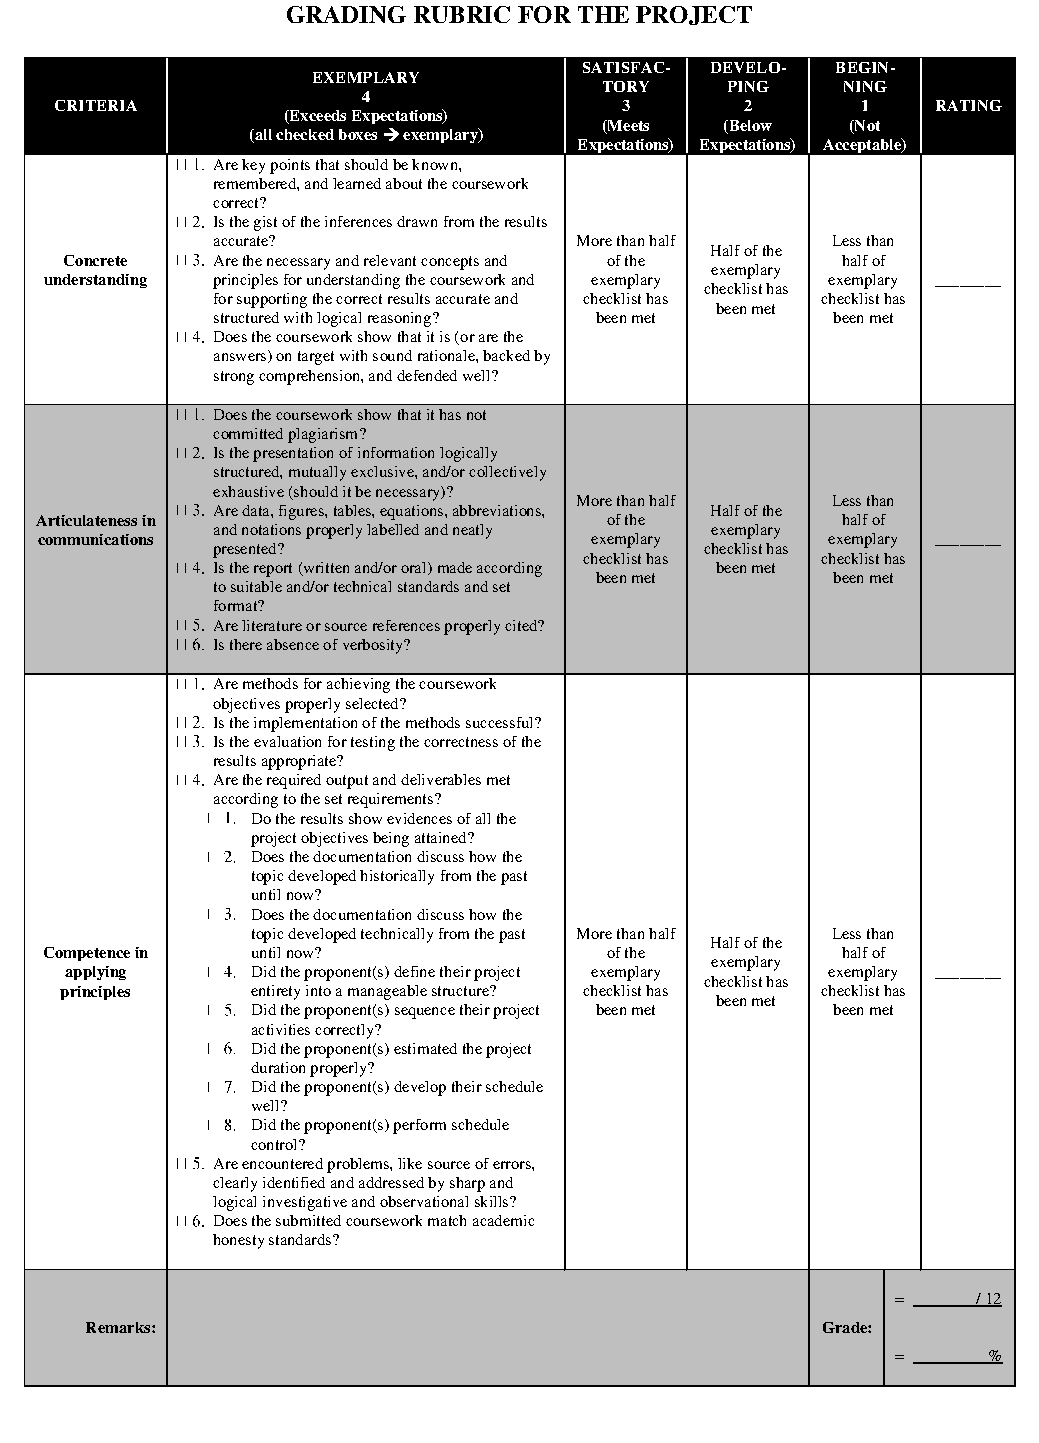
\includegraphics[width=\textwidth]{rubric} 
\end{figure*}
\cleardoublepage

\end{document}